With an understanding of the EoR and the challenges of observing it, we turn to
some of the intensity mapping experiments that look to constrain reionization. Several
instruments, such the Low Frequency Array (LOFAR; \cite{2013A&A...550A.136Y}), the Donald C. Backer Precision Array
for Probing the Epoch of Reionization (PAPER; \cite{2010AJ....139.1468P}), and the Murchison Widefield Array (MWA; \cite{2013PASA...30....7T}),
have come online to help constrain reionization through the detection of
neutral hydrogen emission between early stars and galaxies. Each of these approached the problem of detecting
EoR fluctuations in their own way, but so far none have been successful at
detecting the EoR signal. However, the lessons learned from each of these experiments
have been used to help inform the construction of a next-generation 21\,cm experiment,
the Hydrogen Epoch of Reionization Array.

\begin{figure}[ht]
	\centering
	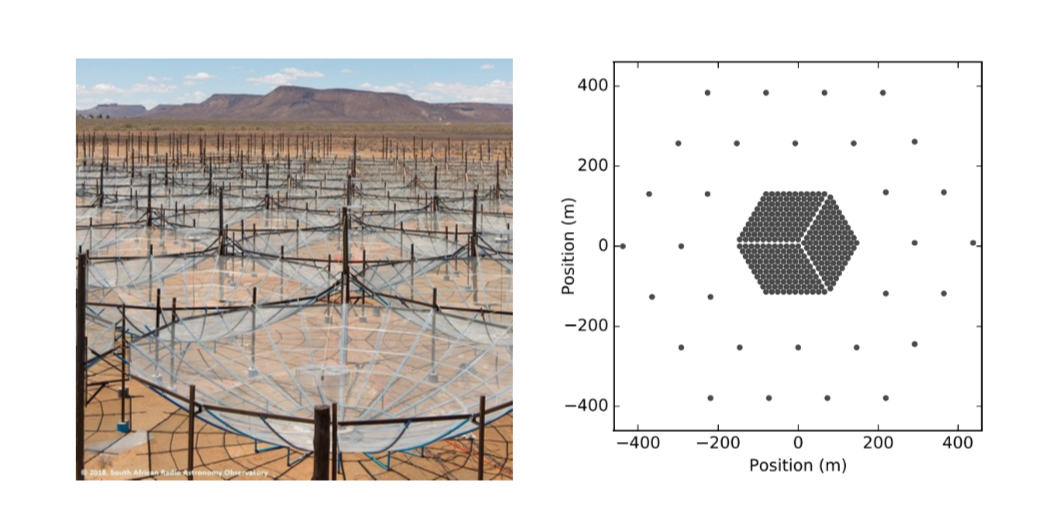
\includegraphics[width=1\textwidth]{intro/hera_layout.png}
	\caption[HERA Image and Layout]{Left: An image of HERA as of late 2017. Right: A map of
					 the full layout of HERA. The final array will contain a total of 350, 14 m dishes.}
	\label{fig:hera_layout}
\end{figure}

The Hydrogen Epoch of Reionization Array (HERA; \cite{2017PASP..129d5001D}) is
a radio interferometer built in South Africa whose primary science goal is
the study of large-scale structure through the power spectrum of the redshifted 21\,cm
line. When complete, HERA will be composed of a total of 350, 14-meter dishes, 320
of which will be tightly compacted in a hexagonal core with the remaining 30 placed
outside the core to increase its imaging capabilities (Figure \ref{fig:hera_layout}). This dense arrangement of
dishes was designed specifically to avoid bright radio foregrounds 4-5 orders of
magnitude brighter than the cosmological 21\,cm signal. With a greater collecting
area and a foreground avoidance strategy superior to previous experiments, HERA
expects to measure EoR fluctations at large-scales with high sensitivity and
provide the first constraints on reionization-era astrophysical parameters using
the 21\,cm line. Construction is currently on-going to complete the array. It is estimated
that HERA will be constructed and begin taking data with the full array in late 2020.
